\documentclass{article}
\setlength{\oddsidemargin}{0.25 in}
\setlength{\evensidemargin}{-0.25 in}
\setlength{\topmargin}{-0.6 in}
\setlength{\textwidth}{6.5 in}
\setlength{\textheight}{8.5 in}
\setlength{\headsep}{0.75 in}
\setlength{\parindent}{0 in}
\setlength{\parskip}{0.1 in}
\usepackage{amsmath,amsfonts,graphicx}
\usepackage{tikz}
\usepackage{epsfig}
\usepackage{filecontents}
\usepackage{pgfplots, pgfplotstable}
\usepackage{mathtools}
\usepackage{breqn}
\usepackage{graphicx}
\usepackage{subcaption}
\usepgfplotslibrary{statistics}

\newcounter{lecnum}
\renewcommand{\thepage}{\thelecnum-\arabic{page}}
\renewcommand{\thesection}{\thelecnum.\arabic{section}}
\renewcommand{\theequation}{\thelecnum.\arabic{equation}}
\renewcommand{\thefigure}{\thelecnum.\arabic{figure}}
\renewcommand{\thetable}{\thelecnum.\arabic{table}}

\newcommand{\lecture}[4]{
  \pagestyle{myheadings}
  \thispagestyle{plain}
  \setcounter{lecnum}{#1}
  \setcounter{page}{1}
  \noindent
  \begin{center}
    \framebox{
      \vbox{\vspace{2mm}
        \hbox to 6.28in { {\bf Analysis of Uncertainties
	    \hfill Fall 2014} }
        \vspace{4mm}
        \hbox to 6.28in { {\Large \hfill Lecture #1: #2  \hfill} }
        \vspace{2mm}
        \hbox to 6.28in { {\it Lecturer: #3 \hfill Notes by: #4} }
        \vspace{2mm}}
    }
  \end{center}
  \markboth{Lecture #1: #2}{Lecture #1: #2}
  \vspace*{4mm}
}

\renewcommand{\cite}[1]{[#1]}
\def\beginrefs{\begin{list}%
    {[\arabic{equation}]}{\usecounter{equation}
      \setlength{\leftmargin}{2.0truecm}\setlength{\labelsep}{0.4truecm}%
      \setlength{\labelwidth}{1.6truecm}}}
\def\endrefs{\end{list}}
\def\bibentry#1{\item[\hbox{[#1]}]}

\newtheorem{theorem}{Theorem}[lecnum]
\newtheorem{lemma}[theorem]{Lemma}
\newtheorem{proposition}[theorem]{Proposition}
\newtheorem{claim}[theorem]{Claim}
\newtheorem{corollary}[theorem]{Corollary}
\newtheorem{definition}[theorem]{Definition}
\newenvironment{proof}{{\bf Proof:}}{\hfill\rule{2mm}{2mm}}

\newcommand\E{\mathbb{E}}

\begin{document}
\lecture{3}{28 October 2014}{Prof. Kate Scholberg}{Douglas Davis}
\section{Estimating means \& errors from data}
In lecture one, we stated the following connection:
\begin{center}
  \begin{tabular}{ c | c }
    \emph{sample} quantities & \emph{truth}/parent quantities                                            \\
    \hline\hline
    $\overline{x}$           & $\mu$                                                                     \\
    $s^2$                    & $\sigma^2$                                                                \\
    \hline    
  \end{tabular}
\end{center}
In many common situations the parent is a Gaussian or Poisson distribution
(Poisson for low mean, low rate). For now let's assume we have a parent which
is Gaussian. The probability $dQ$ of measuring between possibility $x$ and
$x+dx$ is given by
\begin{align}
  dQ = \frac{1}{\sigma\sqrt{2\pi}}\exp\left[
  {-\frac{1}{2}\left(\frac{x-\mu}{\sigma}\right)^2}\right]dx.
  \label{eq:dq}
\end{align}
Let's say we our particular measurements are $x_i$ and the probability of
measuring $P_i$ is $P(x_i)$. We'll say that each $x_i$ has the same $\mu$
and $\sigma$. Our set is
\begin{align*}
  \{x_i\}: \{x_1,x_2,...,s_N\}.
\end{align*}
Using the notation $\mu = \text{truth distribution}$ and
$\mu' = \text{best estimate}$, let's work out $\mu'$ assuming
that $\sigma' = \sigma$ and is constant. We start by defining:
\begin{align}
  P_i(\mu_i)                 & = P(x_i|\mu_i), \text{ probability of getting } x_i \text{ given } \mu_i, \\
  P_i(\mu')                  & = \frac{1}{\sigma\sqrt{2\pi}}\exp\left[{-\frac{1}{2}\left(\frac{x_i-\mu'}{\sigma}\right)^2}\right].
\end{align}
We assume all probabilities are independent, therefore all probabilities can be multiplied to gather the probability of getting our entire set, recall that when $A$ and $B$ are independent:
\begin{align*}
  P(AB) = P(A)P(B).
\end{align*}
Therefore, given $\mu'$ the probability of getting $x_1\, ...\, x_N$ (our collection) is:
\begin{align}
  P(\mu') = \prod_i^N P_i(\mu') \equiv \text{``Likelihood''}.
  \label{eq:like}
\end{align}
For our current scenario:
\begin{align}
  P(\mu') = \prod_i^N P_i(\mu') = \left(\frac{1}{\sigma\sqrt{2\pi}}\right)^N\exp\left[-\frac{1}{2}\sum_i^N \left(\frac{x_i-\mu'}{\sigma}\right)^2\right].
  \label{eq:full_like}
\end{align}
To get the best estimate for the mean we need to ``maximize the likelihood.'' This is called the method of maximum likelihood. To do this, it is clear that we need to minimize the sum in equation~\ref{eq:full_like}. We'll minimize as a function of $\mu'$:
\begin{align*}
  \frac{d}{d\mu'}\left[\frac{1}{2}\sum_i^N\left(\frac{x-\mu'}{\sigma}\right)^2\right] = 0 = \sum_i^N\left(\frac{x_i-\mu'}{\sigma^2}\right) \quad \rightarrow \quad \sum_i^N x_i = \sum_i^N \mu' = N\mu'.
\end{align*}
This yields the familiar mean of the sample:
\begin{align}
  \mu' = \frac{1}{N}\sum_i^Nx_i.
  \label{eq:main_mean}
\end{align}
Therefore, using the general maximum likelihood method, we arrive at the simple mean of the sample maximizes the likelihood and is therefore the best estimate of the mean. Next, we will work out the uncertainty on $\mu'$. It's a common mistake to take $\sigma$ as the uncertainty on the mean, but this is actually incorrect -- we have more knowledge about the mean than that (the uncertainty is less than $\sigma$). We'll take our error propagation from lecture one. For some variable $y$ as a function of $u,v,w... = \{\alpha_i\}$:
\begin{align}
  \sigma_y^2 = \sum_{\alpha} \left|\frac{\partial f}{\partial x_{\alpha}}\right|^2\sigma_{\alpha}^2 + \text{ covariant terms}.
\end{align}
Here we are assuming no correlation so no covariant terms. Now we identify $\mu'$ as $y$ and the $x_i$'s as the $u,v,w...$ set.
\begin{align*}
  \sigma_{\mu'}^2 = \sum_i^N \sigma_i^2 \left|\frac{\partial \mu'}{\partial x_i}\right|^2 =  \sigma^2\sum_i^N \left|\frac{\partial \mu'}{\partial x_i}\right|^2,
\end{align*}
for constant $\sigma_i = \sigma$ (all $x_i$ drawn from same sample).
\begin{align*}
  \frac{\partial \mu'}{\partial x_i} = \frac{1}{N},
\end{align*}
therefore:
\begin{align*}
  \sigma_{\mu'}^2 = \sigma^2\sum_i^N \frac{1}{N^2} = \sigma^2N\frac{1}{N^2} = \frac{\sigma^2}{N}.
\end{align*}
And now we've arrived at the uncertainty on the mean:
\begin{align}
  \sigma_{\mu'} = \frac{\sigma}{\sqrt{N}}.
  \label{eq:main_unc}
\end{align}
Now we suppose that $\sigma_i$'s are not all constant $\sigma$. We begin by just taking equation~\ref{eq:full_like} and using $\sigma_i$ for $\sigma$. Now it is iterated over in the product.
\begin{align}
  P(\mu') = \prod_i^NP_i(\mu') = \left(\frac{1}{\sigma_i\sqrt{2\pi}}\right)^N\exp\left[-\frac{1}{2}\sum_i^N\left(\frac{x_i-\mu'}{\sigma_i}\right)^2\right].
\end{align}
We again maximize the likelihood by minimizing the sum in the exponential, now with unique $\sigma_i$:
\begin{align*}
  \frac{d}{d\mu'}\frac{1}{2}\sum_i^N\left(\frac{x_i-\mu'}{\sigma_i}\right)^2 = 0 = \sum_i^N \frac{x_i-\mu'}{\sigma^2} \quad \rightarrow \quad \sum_i^N \frac{x_i}{\sigma_i^2} - \mu'\sum_i^N \frac{1}{\sigma^2} = 0.
\end{align*}
We arrive at:
\begin{align}
  \mu' = \frac{\sum_i^N\frac{x_i}{\sigma_i^2}}{\sum_i^N\frac{1}{\sigma_i^2}}.
  \label{eq:vary_mean}
\end{align}
And the variance of the estimate of the mean (uncertainty on the mean):
\begin{align}
  \sigma_{\mu'}^2 = \frac{1}{\sum_i^N\frac{1}{\sigma_i^2}}.
  \label{eq:vary_unc}
\end{align}
Notice that if $\sigma_i\rightarrow \text{constant } \sigma$ equations~\ref{eq:vary_mean}~\&~\ref{eq:vary_unc} just go to equations~\ref{eq:main_mean}~\&~\ref{eq:main_unc}, respectively.

Let's take a minute to talk about Poisson. For Poisson distributions $\sigma \rightarrow \sqrt{\mu}$. When we think Poisson we think low rate counting, for example: a low number of events in some $\Delta t$. Let $\mu_t$ be the mean number of events in $\Delta t$. The Poisson distribution:
\begin{align}
  P(x;t) \rightarrow P(x;\mu) = \frac{\mu^xe^{-\mu}}{x!},
\end{align}
for $x = 0, 1, 2,...$ . Imagine $N$ measurements (for $\mu \geq 10$ this would $\sim$ Gaussian).
\begin{align}
  \mu_t \sim \overline{x}_t,
\end{align}
$\overline{x}_t$ is the best estimate of $\mu_t$, the best estimate of the variance is
\begin{align}
  \sigma_t = \sqrt{\mu_t} \sim \sqrt{\overline{x}_t}.
\end{align}
This is the spread. The error on the mean is
\begin{align}
  \sigma_{t\mu} = \frac{\sigma_t}{\sqrt{N}} \sim \sqrt{\frac{\overline{x}}{N}}.
\end{align}
We'll look at a quick example: Take $N = 4$, with measurements 3, 4, 7, and 2.
\begin{align*}
  \mu_t                    & = \overline{x}_t = \frac{1}{4}\times(3 + 4 + 7 + 2) = 4              \\
  \sigma_t                 & = 2                                                                  \\
  \sigma_{t\mu}            & = \sqrt{4/4} = 1                                                     \\
  \text{therefore, } \mu_t & = 4 \pm 1
\end{align*}
\section{Error Matrices Introduction}
Error matrices are helpful for understanding correlations. consider two variables $u,\,v$ -- each is a Gaussian with $\sigma_u,\,\sigma_v$ and $\mu_u = \mu_v = 0$ (binormal).
\begin{align*}
  P(u) = \frac{1}{\sigma_u\sqrt{2\pi}}e^{-u^2/2\sigma_u^2} \qquad P(v) = \frac{1}{\sigma_v\sqrt{2\pi}}e^{-v^2/2\sigma_v^2}.
\end{align*}
The uncorrelated combination (probability of $u$ and $v$):
\begin{align}
  P(uv) = P(u)P(v) = \frac{1}{2\pi\sigma_u\sigma_v}\exp\left[-\frac{1}{2}\left(\frac{u^2}{\sigma_u^2}+\frac{v^2}{\sigma_v^2}\right)\right].
\end{align}
Let's focus on the $\left(u^2/\sigma_u^2 + v^2/\sigma_v^2\right)$ term in the exponential. If the sum of this term is equal to one, then the probability is goes down by a factor of $e^{-1/2}$. The term equal to 1 is also the equation of an ellipse.
\begin{align}
  \frac{u^2}{\sigma_u^2}+\frac{v^2}{\sigma_v^2} = 1
  \label{eq:ell}
\end{align}
Figure~\ref{fig:tri}a shows the ellipse and Figure~\ref{fig:tri}b shows the ellipse overlayed with a chosen value of $u$. Equation~\ref{eq:ell} can be written in matrix form:
\begin{align*}
  \begin{pmatrix}
    u                      & v
  \end{pmatrix}
  \underbrace{
    \begin{pmatrix}
      1/\sigma_u^2         & 0                                                                    \\
      0                    & 1/\sigma_v^2
  \end{pmatrix}}_{M^{-1}}
  \begin{pmatrix}
    u                                                                                             \\
    v
  \end{pmatrix}
  = 1,
\end{align*}
where
\begin{align}
  M = 
  \begin{pmatrix}
    \sigma_u^2             & 0                                                                    \\
    0                      & \sigma_v^2
  \end{pmatrix}.
\end{align}
$M$ above represents uncorrelated $u$ and $v$. In general the matrix elements of $M$ are represented as:
\begin{align}
  M_{ij} = \left\langle\left(w_i - \overline{w}_i\right)\left(w_j-\overline{w}_j\right)\right\rangle,
\end{align}
where $w_i,w_j$ in our matrix above is either $u$ or $v$. Therefore:
\begin{align*}
  \text{for } i = j        & \rightarrow \left\langle(u-\overline{u})^2\right\rangle = \sigma_u^2 \\
                           & \rightarrow \left\langle(v-\overline{v})^2\right\rangle = \sigma_v^2 \\
  \text{for } i \neq j     & \rightarrow \left\langle(u-\overline{u})(v-\overline{v})\right\rangle = \sigma_{uv}^2 =
  \lim_{N\rightarrow\infty}\frac{1}{N}\sum_k^N\left(u_k - \overline{u}\right)\left(v_k - \overline{v}\right)
\end{align*}
Now we'll wrap up with a quick example: suppose we have uncorrelated $u$ and $v$ where:
\begin{align*}
  u'                       & = u\cos\theta - v\sin\theta                                          \\
  v'                       & = u\sin\theta + v\cos\theta
\end{align*}
Which allows us to write an equation similar in form to equation~\ref{eq:ell}, with $a,b,c$ some constants:
\begin{align*}
  \frac{u^{\prime 2}}{a} + \frac{v^{\prime2}}{b} + \frac{u'v'}{c} = 1
\end{align*}
Now this equation is no longer a standard ellipse with a major and minor axis, it has some tilt to it, which we show in Figure~\ref{fig:tri}c. The most likely values for $u$ and $v$ are no longer the easy find at the $0$ for the partner variable. This will continue in the next lecture.
\begin{figure}
  \centering
  \begin{subfigure}{.25\textwidth}
    \centering
    \begin{tikzpicture}[scale=.7,
        grid/.style={
          color=white!50!black,stealth-stealth
        }
      ]
      \node (o) at (0,0) {};
      \draw [grid] (-2.2,0) -- (2.2,0) node [below,xshift=-6pt] {$u$};
      \draw [grid] (0,-2.7) -- (0,2.7) node [right,yshift=-6pt] {$v$};
      \draw (o) ellipse [start angle=0, end angle=360, x radius=1.3, y radius=2.0];
      \draw [-stealth] (o)++(5pt, 5pt) -- +(0,1) node [midway, right] {$\sigma_v$};
      \draw [-stealth] (o)++(5pt,-5pt) -- +(1,0) node [midway, below] {$\sigma_u$};  
    \end{tikzpicture}
    \caption{}
  \end{subfigure}
  ~
  \begin{subfigure}{.25\textwidth}
    \centering
    \begin{tikzpicture}[scale=.7,
        grid/.style={
          color=white!50!black,stealth-stealth
        }
      ]
      \node (o) at (0,0) {};
      \draw [grid] (-2.2,0) -- (2.2,0) node [below,xshift=-6pt] {$u$};
      \draw [grid] (0,-2.7) -- (0,2.7) node [right,yshift=-6pt] {$v$};
      \draw (o) ellipse [start angle=0, end angle=360, x radius=1.3, y radius=2.0];
      \draw [-stealth] (o)++(5pt, 5pt) -- +(0,1) node [midway, right] {$\sigma_v$};
      \draw [-stealth] (o)++(5pt,-5pt) -- +(1,0) node [midway, below] {$\sigma_u$};  
      \draw [grid,dashed,color=blue!70] (-.5,-2.7) -- (-.5,2.7);
    \end{tikzpicture}
    \caption{}
  \end{subfigure}
  ~
  \begin{subfigure}{.25\textwidth}
    \centering
    \begin{tikzpicture}[scale=.7,
        grid/.style={
          color=white!50!black,stealth-stealth
        }
      ]
      \node (o) at (0,0) {};
      \draw [grid] (-2.2,0) -- (2.2,0) node [below,xshift=-6pt] {$u$};
      \draw [grid] (0,-2.7) -- (0,2.7) node [right,yshift=-6pt] {$v$};
      \draw (o) ellipse [start angle=0, end angle=360, x radius=1.3, y radius=2.0,rotate=45];
      \draw [-stealth] (o)++(5pt, 5pt) -- +(0,1) node [midway, right] {$\sigma_v$};
      \draw [-stealth] (o)++(5pt,-5pt) -- +(1,0) node [midway, below] {$\sigma_u$};
    \end{tikzpicture}
    \caption{}
  \end{subfigure}
  \caption{For (a), (b), and (c), the black ellipse is called the \emph{contour of equal probability}. In (b), the blue dash represents a chosen $u$, and here the maximum probability would be at $v = 0$. In (c), the ellipse has been rotated by some angle $\theta$, and at some chosen $v$ or $u$, the maximum probability is not longer at $u=0$ and $v=0$, respectively.}
  \label{fig:tri}
\end{figure}

\end{document}
